\documentclass{article}
\usepackage[T1]{fontenc}
\usepackage[utf8]{inputenc}
\usepackage[table]{xcolor}
\usepackage{hyperref}
\usepackage{mathtools}
\usepackage{graphicx} 
\usepackage{titlesec}
\usepackage{float}
\usepackage{tabularx,booktabs,caption,ragged2e}
\usepackage{biblatex}
\usepackage{eurosym}
\usepackage{amsmath , amsfonts, amssymb}
\usepackage{longtable}
\usepackage{adjustbox}
\addbibresource{bibliographie.bib}
\setlength{\parindent}{0pt}
\captionsetup{skip=0.333\baselineskip}

\begin{document}
\section{Résumé}
\section{Introduction} 
Malgré l'augmentation du nombre de logements, les inégalités ne cessent d'aug-menter. D'après l'Insee le nombre de logements à presque doublé alors que la population n'a augmenté que 
de 37\%\cite{evolution_hab}. La hausse des inégalités et la baisse du pouvoir d'achat étant au cœur de l'actualité. Lorsque en 2018, les dépenses de loyers pesaient 6.1\% dans l'IPC\cite{ipc_loyer}, ou bien que 24\% des ménages détiennent plus de la moitié des logements possédés\cite{part_appart}. Nous avons trouvé bon d'essayer de modéliser économétriquement la part des locataires en résidences principales. C'est à dire, la part des personnes vivant en résidence principale et qui n'en sont pas propriétaires. La problématique est la suivante :
Quels sont donc les principaux facteurs expliquant la part de locataire en résidence principale dans les départements Français? 

\section{Données utilisées}
Les données utilisées ont été sélectionnés dans la base de l'INSEE pour l'année 2019 sur l'ensemble des départements. Cependant certaines valeurs n'étant pas disponibles pour les départements d'outre-mer,
L'étude se portera uniquement sur les départements de France métropolitaine.
\subsection{Variable expliquée}
La variable dépendante est :
\begin{itemize}
    \item $locataire$ : la part de locataires en résidences principales, celle-ci comprend les locataires du parc public (HLM) ainsi que ceux du parc privé.
\end{itemize}
En moyenne, le taux de locataires dans un département de France métropolitaine est de 36,47 \%, avec pour minimum 24,3\% (Creuse) et pour maximum 61,7\%(Paris).
L'écart type de la part de locataires, est assez élevé à 6,77\%. Cela dénote une certaine hétérogénéité entre les différents départements Français.
\subsection{Variables explicatives}
Au total, sept variables sous forme de taux ont été choisies pour essayer d'expliquer la part de locataires.
\begin{itemize}
    \item $dipsup$ : La part des diplômés d'un BAC+5 ou plus, le niveau de diplôme conditionne la catégorie socioprofessionnelle d'un travailleur et par extension son salaire
        . La part des hauts diplômés peut donc être un bon indicateur de niveau de vie.
    \item $appart$ : La part d'appartements dans le total des logements. Le parc locatif Français comprend une majorité d'appartements\cite{part_appart}, cette variable pourrait donc
        avoir un fort impact positif sur la part de locataires.
    \item $chomage$ : Le taux de chômage annuel moyen. Le taux de chômage peut être un bon indicateur de richesse, un agent au chômage aura une plus faible chance de pouvoir contracter
        un prêt que un agent n'étant pas au chômage, et par conséquent aura plus tendance à être locataire.
    \item $urba$ : La part de la population vivant dans une unité urbaine, permet de donner un bon aperçu de la proportion d'habitants urbains.
    \item $persagee$ : La part des personnes âgées de 65 ans ou plus dans la population. Cette variable devrait avoir un effet négatif sur la part de locataires, car plus l'age augmente, plus
        un agent est susceptible d'accumuler du capital et a utiliser ce dernier dans l'acquisition d'un bien immobilier. En fonction de l'age, la part de propriétaires augmente grandement.\cite{part_appart}
    \item $pauvrete$ : Le taux de pauvreté. Comme indicateur de richesse, en effet, la pauvreté a plus tendance a toucher les locataires.\cite{pauvrete_locataires}
    \item $jeune$ : La part des personnes âgées de moins de 25 ans dans la population. Au contraire des personnes âgées de plus de 25 ans, cette variable devrait avoir un effet positif sur
        la variable dépendante.
    \end{itemize}
\begin{table}[H]
    \centering
    \caption{Statistiques sur les variables explicatives}
    \begin{tabular}{l*{1}{|cccc}}
                \toprule
                Variable    &    Moyenne &Écart Type& Minimum&     Maximum\\
                \midrule
                dipsup      &    8,14&    5,10&         3,8&        39,5\\
                appart      &    35,86&    17,26&        12,9&        96,9\\
                chomage     &    7,55&    1,47&         4,3&        12,3\\
                urba        &    68,07&    17,62&        21,4&         100\\
                persagee    &    22,17&    3,94&        11,9&        30,1\\
                pauvrete    &    14,37&    2,99&         9,1&        27,9\\
                jeune       &    27,99&    2,98&        21,6&        35,4\\
                \bottomrule
    \end{tabular}
\end{table}
Et une variable indicatrice a été codée.
\begin{itemize}
    \item $ville$ : Variable indicatrice, prend la valeur 1 si le département comprend une des 15 villes les plus peuplées de France, 0 sinon. Cette variable permet de distinguer les
        départements avec grande ville. Étant donné que les données sur les prix immobiliers par départements ne sont pas disponibles, on peut émettre l'hypothèse que l'immobilier dans
        les grandes villes est élevé, alors cette variable peut être utilisée comme mesure des coûts de l'immobilier.
\end{itemize}
Une fois les variables sélectionnées, une matrice de corrélation des variables peut être dressée.
\begin{table}[H]
    \caption{Matrice du coefficient de corrélation entre les variables}
    \adjustbox{max width=\textwidth}{%
    \centering
    \begin{tabular}{l*{1}{|ccccccccc}}
        \toprule
                  &locataire        &   dipsup      &   appart         &  chomage         &     urba         & persagee         & pauvrete         &    jeune         & ville\\
        \midrule
        locataire &        1        &               &                  &                  &                  &                  &                  &                  &\\
        dipsup    &    0,736        &        1      &                  &                  &                  &                  &                  &                  &\\
        appart    &    0,849        &    0,789      &        1         &                  &                  &                  &                  &                  &\\
        chomage   &    0,300        &  -0,0646      &    0,125         &        1         &                  &                  &                  &                  &\\
        urba      &    0,780        &    0,644      &    0,783         &    0,319         &        1         &                  &                  &                  &\\
        persagee  &   -0,729        &   -0,552      &   -0,630         &  -0,0944         &   -0,695         &        1         &                  &                  &\\
        pauvrete  &    0,315        &  -0,0775      &    0,111         &    0,755         &    0,127         &   0,0374         &        1         &                  &\\
        jeune     &    0,643        &    0,384      &    0,476         &    0,150         &    0,649         &   -0,937         &  -0,0311         &        1         &\\
        ville     &   0.4998        &   0.4039      & 0.4285           & 0.0906           &0.4574            &  -0.2772         &   0.0464         &    0.2840        &1.0000\\
        \bottomrule
        \end{tabular}}
\end{table}
\newpage
\section{Modélisation}
\subsection{Modèle initial}
\subsubsection{Spécification du modèle}
Le premier modèle est formulé de la sorte : 
\begin{equation}
\begin{split}
		locataire_i =  \beta_1 &+ \beta_2dipsup_i + \beta_3jeune_i + \beta_4persagee_i \\
						&+ \beta_5appart_i + \beta_6chomage_i + \beta_7urba_i \\
						&+ \beta_8pauvrete_i + \beta_9ville_i + \varepsilon_i 
\end{split}
\end{equation}
\subsubsection{Interprétation des résultats }
On estime par la méthode des moindres carrés ordinaires les coefficients de l'équation précédente.
\begin{table}[H]
\centering
\caption{Première regression}
\begin{tabular}{l*{1}{cc}}
\toprule
Variable            & Coefficient         &  Écart-Type\\
\midrule
Constante &  -0,5843203 &  13,0103\\
dipsup	& 0,3628173	& 0,0822579\\
jeune  & 0,7166451 & 0,2818662\\
persagee&  -0,0439146 & 0,2321425\\
appart& 0,1539156 & 0,0297159\\
chomage& -0,1594068 & 0,2771842\\
ubra& -0,0037748 & 0,0278766\\
pauvrete& 0,739118& 0,1265662\\
ville &   2,175549  &  0,747542\\
\midrule
N&          96         &            \\
SCE & $3917,00559$ \\
SCR & $442,199351$ \\
SCT & $4359,20494$ \\
\bottomrule
\end{tabular}
\end{table}
Le modèle s'écrit alors : 
\begin{equation*}
    \begin{split}
			\hat{locataire}_i =  -0,58 &+ 0,36 \times dipsup_i + 0,72 \times jeune_i - 0,04 \times persagees_i \\
            &+ 0,15 \times appart_i -0,16 \times chomage_i - 0,004 \times urba_i \\ 
			& + 0,74 \times pauvrete_i + 2,18 \times ville_i \\
    \end{split}
\end{equation*}
Le coefficient de détermination $R^{2}$ est calculé.
\begin{equation*}
    R^{2} = \frac{SCE}{SCT} = \frac{3917,00559}{4359,20494} = 0,8986
\end{equation*}
Ainsi que le coefficient de détermination ajusté aux nombres de variables.
\begin{equation*}
    \bar{R}^{2} = 1 - \frac{SCR/(N-K)}{SCT/(N-1)} = \frac{442,199351/87}{4359,20494/95} = 0,8892
\end{equation*}
Les deux coefficients sont élevés, cela laisse donc à supposer que l'ajustement de de la regression est de bonne qualité. Cependant, des tests de 
significativité (des paramètres et conjointe), et une étude de la multicolinéarité restent à être menés pour confirmer cela.
\subsubsection{Tests de significativité}
\label{sec:testSigni1}
Dans un premier temps, le test $F$ de significativité conjointe est fait. L'hypothèse nulle, et l'hypothèse alternative de ce test sont telles que :
\begin{equation*}
\begin{split}
    H_0 &: \beta_2 = \beta_3 = \dots \beta_K =0 \\
    H_1 &: \text{Au moins un }\beta_j \neq 0.
\end{split}
\end{equation*}
La statistique de test sous l'hypothèse nulle est distribuée selon une loi $F$ de Fisher.
\begin{equation*}
    F = \frac{SCE/(K-1)}{SCR/(N-K)} \sim F(K-1, N-K)
\end{equation*}
Pour un niveau de test à $\alpha = 5\%$, on compare la statistique calculée au quantile à $95\%$ de la distribution $F$ de Fisher avec 
comme degrés de liberté $8$ et $87$ respectivement au numérateur et au dénominateur. 
\begin{equation*}
    F_{1-\alpha} (K-1, N-K) = F_{0.95}(8, 87) = 2,0466714
\end{equation*}
Après calculs, $F = 96,33$. La statistique est supérieure au seuil, l'hypothèse nulle est rejetée au moins une variable permet d'expliquer le modèle.
\\ \\
Maintenant, il faut déterminer plus précisément quels sont les paramètres estimés significativement différents de 0. Pour cela, un test $t$ de 
significativité est effectué sur sur les $9$ paramètres :
\begin{equation*}
\begin{split}
    H_0 &: \beta_j =0 \\
    H_1 &: \beta_j \neq 0
\end{split}
\end{equation*}
La statistique de test calculée sous l'hypothèse nulle est distribuée selon une loi $t$ de Student : 
\begin{equation*}
    t_{\beta_j} = \frac{\hat{\beta_j}}{s_{\hat{\beta_j}}} \sim t(N-K)
\end{equation*}
Le niveau de test bilatéral est $\alpha = 5\%$ et la statistique en valeur absolue doit être comparée au quantile à $97,5\%$ de la distribution
 $t$ de Student à $88$ degrés de liberté, soit le seuil critique :
\begin{equation*}
    t_{1-\alpha/2}(N-K) = t_{0,975}(87) = 1,9876083 
\end{equation*}
Tous calculs faits, les résultats sont :
\begin{table}[H]
\centering
\caption{Statistique $t$}
\begin{tabular}{l*{1}{c}}
\toprule
Variable            &Statistique $t$\\
\midrule
constante &     -0,04\\
dipsup&         4,41\\
jeune&          2,54\\
persagee&       -0,19\\
chomage&        -0,58\\
urba   &        -0,14\\
pauvrete&       5,84\\
ville &         2,91\\
\bottomrule
\end{tabular}
\end{table}
Les statistiques de test $t_{\beta_1},t_{\beta_4},t_{\beta_6}$ et $t_{\beta_7}$ sont inférieures en valeur en absolue au seuil. L'hypothèse nulle, est
acceptée pour ces paramètres, ils ne sont pas significatifs. Les variables $persagee$, $chomage$ et $urba$ seront donc retirées.

En revanche, $t_{\beta_2}, t_{\beta_3}, t_{\beta_5}, t_{\beta_8}$ et $t_{\beta_7}$ sont supérieures en valeur absolue au seuil critique de $1,99$. On rejette l'hypothèse nulle pour ces paramètres
ils sont significatifs, les variables $dipsup$, $jeune$, $appart$, $pauvrete$ et $ville$ permettent d'expliquer en partie $locataire$
\subsubsection{Etude de la multicolinéarité}
Une corrélation forte entre plusieurs variables explicatives peut induire une présence de multicolinéarité dans le modèle. Un calcul du VIF est fait pour chacune des variables.
\begin{table}[H]
\centering
\caption{Facteur d'inflation de la variance}
\begin{tabular}{l*{1}{c}}
\toprule
Variable            &         VIF\\
\midrule
persagee &     15,60  \\
jeune &    13,22 \\
appart &     4,91 \\
urba &    4,51\\
dipsup &   3,29\\
chomage &      3,10 \\
pauvrete &      2,67\\
ville &   1,39\\
\bottomrule
\end{tabular}
\end{table}
Il y a de la multicolinéarité dans le modèle, les variables $jeune$, $persagee$ et $appart$ ont un vif
élevé, les deux dernières seront retirées du modèle afin de traiter la multicolinéarité.
\subsection{Modèle final}
Un second modèle est formulé à la suite des résultats précédents. Ce modèle est tel que :
\begin{equation*}
    \begin{split}
            locataire_i =  \beta_1 &+ \beta_2dipsup_i + \beta_3jeune_i + \beta_4pauvrete_i + \beta_5ville_i+\varepsilon_i 
    \end{split}
\end{equation*}
Les paramètres du modèle sont estimés grace aux MCO.
\begin{table}[H]
\centering
\caption{Regression finale}
\label{table:secondeReg}
\begin{tabular}{l*{1}{ccc}}
\toprule
Variable            & Coefficient&  Écart-type&Statistique t\\
\midrule
constante      &   -9,171721&    3,132582&   -2,39\\
dipsup&    0,7317861 &    0,0619359&    11,82\\
jeune  &     0,910416 &    0,100601&    9,05\\
pauvrete&    0,8258328 &     0,0923714 &   8,94\\
ville &   2,717385 &  0,8330725   &  3,26 \\
\midrule
$N$       &          96& SCE & 3710,78643           \\
$R^{2}$ & 0,8513 &       SCR & 648,418512   \\ 
$\bar{R}^2$ & 0,8447 &   SCT & 4359,20494 \\ 
\bottomrule
\end{tabular}
\end{table}
\subsubsection{Interprétation des résultats}\label{sec:result}
Les trois variables explicatives ont un effet positif sur la part de locataires en résidence principale. L'effet marginal de chaque variable peut être étudié, pour cela,
il suffit de dériver le modèle partiellement par rapport a une des variables pour connaître son effet marginal.
\begin{align*}
    &\frac{\partial locataire}{\partial dipsup} = \hat{\beta_2} \simeq 0,73 & &\frac{\partial locataire}{\partial jeune} = \hat{\beta_3} \simeq 0,91 &\frac{\partial locataire}{\partial pauvrete} = \hat{\beta_4} \simeq 0,83
\end{align*}
Par exemple l'augmentation de la part de diplômés BAC+5 ou plus de 1 point entraînera une augmentation de la part de locataire de 0.73 points toutes choses étant égales par ailleurs.
L'effet le plus fort est l'effet de la population de moins de 25 ans, son effet marginal est presque un pour un. Ce résultat semble logique, puisque les populations jeunes sont très peu
propriétaires\cite{insee_portrait_social}.
\\
D'autre part, les personnes vivant sous le seuil de pauvreté sont moins enclin à acheter un bien immobilier, la location est donc privilégiée.
\\
En revanche, l'effet marginal de la part de hauts diplômés est surprenant. Il serait simple de penser que cet effet soit négatif, car une personne ayant fait de longues études aura un niveau
de vie supérieur à la moyenne et sera donc plus enclin à acheter un bien immobilier pour y vivre. Or ici, l'effet marginal est positif, la principale cause pourrait être le prix élevé de l'immobilier dans les grandes villes (lieu de travail des diplômés supérieurs) en particulier Paris\cite{prix_immo_paris}. Une autre cause pourrait être une mobilité accrue des diplômés
supérieurs comme les cadres. Ou bien une précarité grandissante des diplômés ne trouvant pas de travail\cite{precarite_etude_sup}
L'effet de la présence d'une grande ville dans le département est aussi élevé. Cela confirme que les locataires ont tendance a habiter en ville.
\\ \\
Les coefficients de détermination simple et ajusté sont relativement élevés, la qualité de l'ajustement du modèle est donc bonne. En théorie la
multicolinéarité a été traitée, pour confirmer cela, un calcul des VIF est effectué.
\begin{table}[H]
\centering
\caption{VIF}
\begin{tabular}{l*{1}{c}}
\toprule
Variable            &         VIF\\
\midrule
dipsup  &  1.33  \\
ville   &  1.23  \\
jeune   &  1.20  \\
pauvrete&  1.01  \\
\bottomrule
\end{tabular}
\end{table}
Les trois variables présentes dans le modèle ont un VIF proche de un, elles ne génèrent quasiment pas de multicolinéarité.
\subsubsection{Tests de significativité}
Des tests $t$ de significativité des paramètres sont fait pour déterminer si les paramètres estimés sont significatifs. Le test est le même que dans la
section 2.2.2. Les statistiques $t$ sont dans le tableau ~\ref{table:secondeReg}.
\\
Un niveau de test bilatéral de $\alpha = 5 \%$ est choisis, la statistique  $t$ doit donc être comparée au quantile à  $97,5\%$ de la distribution de
Student à 92 degrés de liberté. Le seuil critique est donc :
\begin{equation*}
t_{0,975}(91) = 1,9863772
\end{equation*}
Toutes les statistiques $t$ des paramètres de la regression sont supérieurs en valeur absolue au seuil critique. $H_0$ est rejetée dans tous les cas.
Tous les coefficients sont significativement différents de 0.
\\
La significativité est aussi testée avec le test $F$ de Fisher comme précédemment dans la section ~\ref{sec:testSigni1}. La statistique $F$ calculée est :
\begin{equation*}
    F =  \frac{3710,78643/4}{648,418512/91} = 130,19
\end{equation*}
Le niveau de test étant $5\%$, cette dernière est comparée au quantile à $95\%$ de la distribution de Fisher. Le seuil est donc :
\begin{equation*}
    F_{0,95}(4,91) = 2,4717915
\end{equation*}
Or $F > 2,472$ l'hypothèse nulle est rejetée, l'ajustement du modèle est de bonne qualité.
\subsubsection{Etude de la normalité des résidus}
Pour que les estimateurs soient de bonne qualité il faut que les erreurs de la régression suivent une loi normale pour cela les résidus sont sont calculés 
et trouvés dans la table ~\ref{appendix:erreurs} des annexes. Ci dessous sont représentés les résidus sous forme d'histogramme, ainsi que, la courbe d'une 
loi normale de même espérance et variance $\mathcal{N}(0,2.61)$.
\begin{figure}[H]
	\centering
	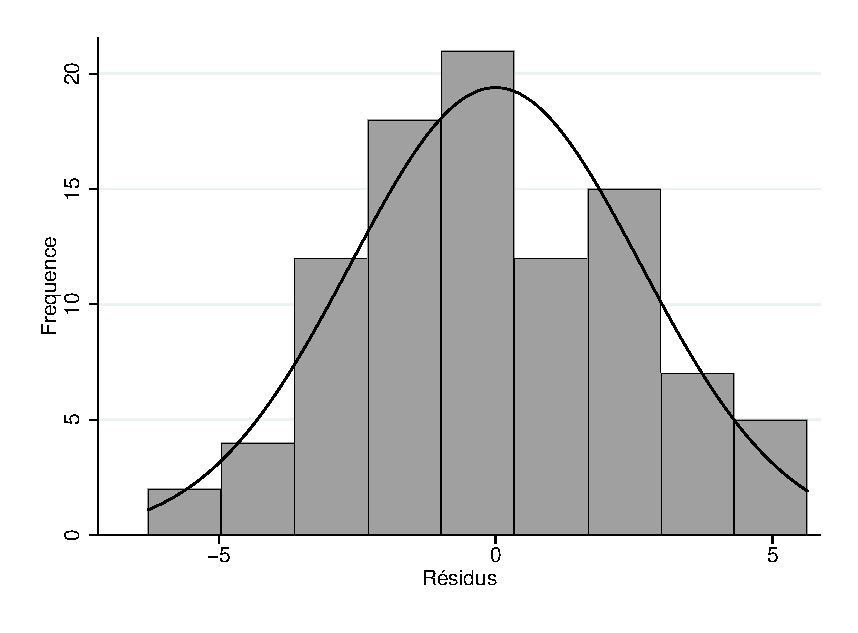
\includegraphics[scale=.6]{Graph.eps}
    \caption{Histogramme des erreurs}
	\label{fig:histogrammeErreur}
\end{figure}
Graphiquement, les résidus semblent suivre la distribution d'une loi normale de meme variance et espérance. L'hypothèse de normalité des erreurs est validée
\subsection{Test d'autocorrélation des résidus}
Dans le cas ou les données sont en coupe instantanée, les résidus sont supposés non-autocorrélés.
\subsubsection{Test sur l'hétéroscédasticité des résidus}
La présence d'hétéroscédasticité dans le modèle pourrait résulter en une mauvaise estimation de la variance des paramètres, dans ce cas là les tests
de significativité de ces paramètres deviendraient invalides. Le test de White d'hétéroscédasticité est réalisé. Les résidus au carré sont estimés par les MCO.
Les hypothèses sont :
\begin{align*}
    &H_0 : \text{Homoscédasticité des erreurs} \\
    &H_1 : \text{Hétéroscédasticité des erreurs}
\end{align*}
La statistique de test est un multiplicateur de Lagrange : $\text{LM} = N \times R^2$ qui est comparé au quantile à $95\%$ (pour un niveau de test à $5\%$) 
de la distribution du khi-deux avec comme degrés de liberté $9$. Les résultats sont représentés dans le tableau ci dessous
\begin{table}[H]
\centering
\caption{Test de White}
\begin{tabular}{l*{1}{c}|{c}{c}}
    \toprule
    $N$ &          96 & $N \times R^2$ & 18,821\\
    $R^{2}$   &0,1961 & $\chi^2_{0.95}(13)$ &22,362 \\
    \bottomrule
\end{tabular}
\end{table}
La statistique de test est inférieure au seuil critique ($N \times R^2 < \chi^2_{0.95}(13)$). L'hypothèse nulle d'homoscédasticité est acceptée.
\\
Le modèle respecte donc bien toutes les hypothèses du modèle linéaire. Le modèle est bien spécifié et les estimateurs sont de bonne qualité.
\section{Conclusion}
Le modèle présenté a eu pour but d'expliquer la part de locataire dans la population par départements. D'après le second modèle estimé et correctement spécifié, il est évident
que la proportion de locataires dans un département est en partie dûe au fait que ce département possède une grande ville. Ainsi, cette dernière attitrera professionnellement une partie
de la population diplômée (comme Paris avec presque 40\% de la population hautement diplômée) qui pour des raisons proposées dans la section ~\ref{sec:result} préféreront la location à
l'achat. D'un autre côté, le taux de pauvreté explique relativement bien la part de locataires, ceci dénote une difficulté d'accès a la propriété pour les personnes vivant en dessous
du seuil de pauvreté. Ainsi pour finir le modèle démontre que l'âge peut être considéré comme un déterminant de la part de locataires.
Certaines variables auraient pû être rajoutées, comme les prix de l'immobilier ou bien la part d'étudiants, car de telles données n'existent pas, ou alors
ne sont pas fournies par l'INSEE au niveau des départements.

dico : VIF = Variance inflation factor
MCO = moindres carrés ordinaires
\newpage
\section{Bibliographie}
\printbibliography

\appendix
\section{Annexes}
Matrice X
Première sortie
Matrice X finale
Sortie finale
Matrice e
Regression auxilière
\end{document}
